% $Header$

\documentclass{beamer}
\mode<presentation>
{
  \usetheme{Warsaw}
  \setbeamercovered{transparent}
}

\usepackage[english]{babel}
\usepackage[latin1]{inputenc}
\usepackage{times}
\usepackage[T1]{fontenc}
\usepackage{graphicx}


\title[Random Graphs]  
{Random Graphs}

\author[Huber] {G.~Huber}

\date[Short Occasion] {18Jul2016 / Final Project Presentation}
\subject{Talks}

\AtBeginSubsection[]
{
  \begin{frame}<beamer>{Outline}
    \tableofcontents[currentsection,currentsubsection]
  \end{frame}
}

\begin{document}

\begin{frame}
  \titlepage
\end{frame}

\begin{frame}{Outline}
  \tableofcontents
\end{frame}

\section{Introduction}

\subsection[Introduction]{Introduction}

\begin{frame}{Random Graph}{A definition}
\begin{quote}
Using the terminology in probability, a random graph is a random variable defined in a probability space
with a probability distribution.[Chung2016]
\par
\vspace{1.0cm}
In layman's terms, we  first put all graphs on $n$ vertices in a lottery box and then the graph we pick 
out of the box is a random graph. (In this case, all graphs are chosen with equal probability.) [Chung2016]
\end{quote}
\end{frame}

\begin{frame}{Random Graphs}{Uses}
\begin{itemize}
\item Random graphs have been used to model the growth of the internet.
\item Random graphs have been used to help analyze social networks.
\item Random graphs have been used to help model epidemiology 
 

\end{itemize}

\end{frame}

\section{Random Graph Models}
\subsection{Erd\"os - R\'enyai model}

\begin{frame}{Introduction}
\begin{itemize}
\item One model introduced by Paul Erd\"os and Alfr\'ed R\'enyai in 1959.
\item A similar model was introduced at the same time by Edgar Gilbert.
\item $G(n,e)$ is a graph chosen at random from all possible graphs with $n$ nodes and $e$ edges.
\item $G(n,p)$ is the graph with $n$ nodes and edges choses from all possible edges with probability $p$.
\end{itemize}
\end{frame}

\begin{frame}{The Algorithm}
\begin{itemize}
\item The algorithm I used to implement the Erd\"os - R\'enyai model is:
\begin{enumerate}
\item Generate $n$ nodes, where $n$ is determined by the user.
\item Generate a set of edges corresponding to all the possible edges in $K_n$.
\item For each edge, generate a uniform random number $[0,1)$ and if this number is less than the probability $p$, also supplied by the user, add the edge to the graph.
\end{enumerate}
\end{itemize}
\end{frame}

\begin{frame}{An example of $G(10,0.15)$}
\begin{figure}
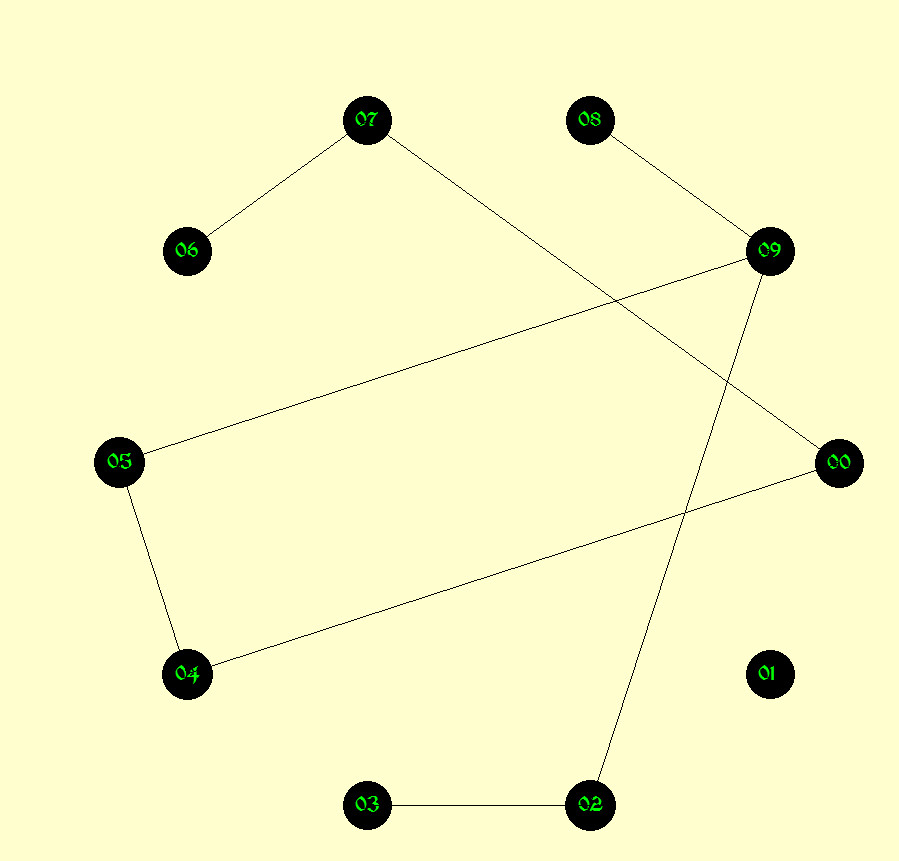
\includegraphics[width= .5\paperwidth]{ERpic.jpg}
\end{figure}
\end{frame}

\begin{frame}{Properties of the graphs produced}
\begin{itemize}
\item On average $G(n,p)$, all nodes have degree close to $(n-1)*p$
\item the value $\frac{ln n}{n}$ is a sharp threshold for connectedness. If p is below this value then there will be disconnected components,
while above this value the graph will be connected. [W2016a]
\item For a 10 node graph, this value is approximately 0.23 
\end{itemize}
\end{frame}

\subsection{Barab\'asi - Albert model}

\begin{frame}{Introduction}
\begin{itemize}
\item A problem with the Erd\"os - R\'enyai model is that all nodes have roughly the same degree.  
\item Many systems (both natural and man-made), for example social networks, Internet connectivity and citation networks do not follow this pattern.
\item Barab\'asi and Albert proposed a model in 1999, with their work on degree distribution on the web.
\item Their model is an example of "preferential attachment"
\item The idea of "preferential attachment" appears to date back to at least 1925.
\end{itemize}
\end{frame}

\begin{frame}{The Algorithm}
\begin{itemize}
\item The algorithm used is:
\begin{enumerate}
\item Begin with a connected network of $m_0$ nodes.  I do this by generating a spanning tree on $K_{m_0}$.
\item Proceed to add new node, $v_j$ to the network one at a time and make $m \leq m_0$ connections to the nodes in the original graph.
\item The probability of an edge being formed between the new node, $v_j$ and an existing node, $v_i$ is given by $p_i = \frac{d(v_i)}{\sum_{v_j \in V(G)}d(v_j)}$
\item Repeat steps (2) and (3) till all the nodes have been added to the graph.
\end{enumerate}
\end{itemize}
\end{frame}

\begin{frame}{The Algorithm}
\begin{itemize}
\item A na\:ive implementation of the above algorithm lead to some problems.
\item The constraint on the number of edges to add is ill-defined.  In other words, how to decide how many edges to add?  I took the 
expedient way out, I hard coded the number of edges at 3.
\item Just generating a uniform random number in [0,1) and comparing it to the probability in step three on the previous slide did admit isolated nodes.
\item On further examination (and research), it appears that the best way to do this is to use a normalize degree distribution. [W2015]
\end{itemize}
\end{frame}

\begin{frame}{Properties of the graphs produced}
\begin{itemize}
\item The degree distribution is 'scale-free'.
\item A 'scale-free' network is a network whose degree distribution follows a power law.  In other words, the fraction, $P(d)$ of nodes having d connections to other nodes is given by $P(d)\space \alpha \space d^{-\gamma}$, where $\gamma \in (2,3)$
\end{itemize}
\end{frame}

\begin{frame}{Example of $m_0$=5, n=5}
\begin{figure}
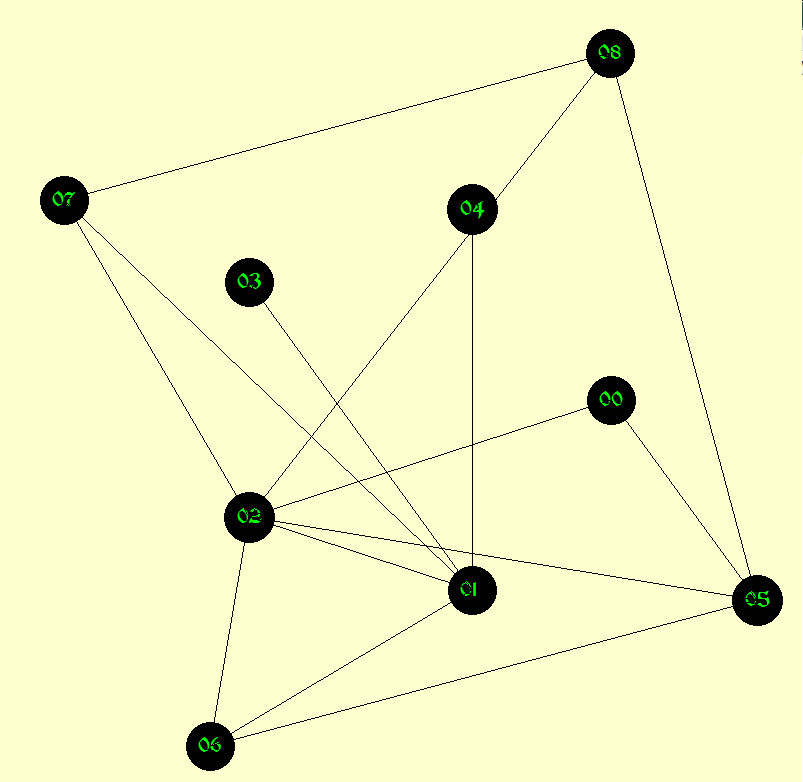
\includegraphics[width= .55\paperwidth]{BApic.jpg}
\end{figure}
\end{frame}


\subsection{Watts - Strogatz model}
\begin{frame}{Introduction}
\begin{itemize}
\item Erd\"os - R\'enyi graphs tend to have short path lengths and low clustering.
\item Certain 'small-world' networks were observed to have both short path lengths and high clustering [W2016b]
\item Small-world networks are networks where nodes are adjacent to only a few nodes, but most nodes are reachable from any other node by a few steps.
\item Small-world networks have the typical distance between arbitrarily chosen nodes to be proportional to the number of nodes in the network
\item The Watts - Strogatz model is designed to produce graphs that exhibit `small-world' properties.
 [wikipedia], {\em i.e.} $d(u,v) \space \alpha log(n)$
\end{itemize}
\end{frame}

\begin{frame}{The Algorithm}
\begin{itemize}
\item The Watts - Strogatz algorithm is:
\begin{enumerate}
\item Given a number of nodes $n$, an average degree, K (assumed to be even), and a 'special parameter' $/beta$
\item Generate a circular lattice of $n$ nodes, where $n$ is the degree of the graph to generate.
\item Attach each node to the K/2 neighbors going clockwise and counter-clockwise
\item For every node $n_i$, take every edge $(n_i, n_j) i < j$ and rewire with a probability $/beta$.  Rewiring is done by replacing $(n_i, n_j)$ with $(n_i, n_k)$ where $k$ is chosen at random from all nodes that avoid multiple edges and self-loops.
\end{enumerate}
\end{itemize}
\end{frame}

\begin{frame}{Properties of the graphs produced}
\begin{itemize}
\item The parameters are expected to follow $ n \gg k \gg ln(n) \gg 1$
\item [W-S]Watts and Strogatz found that L is approximately $\frac{n}{2k} \gg 1$ and the clustering coefficient approaches  $\frac{3}{4}$ as $\beta$ approaches 0.
\item [W-S] Watts and Strogatz showed that L approaches $\frac{ln(n)}{ln(k)}$ and C approaches $\frac{k}{n}$ as $\beta$ approaches 1.
\item We expect $\beta\frac{nK}{2}$ non-lattice edges
\end{itemize}
\begin{figure}
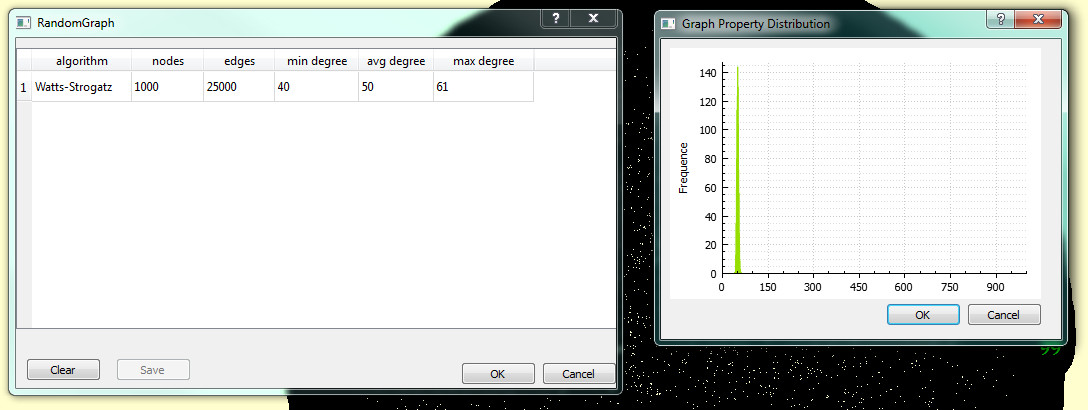
\includegraphics[width= .55\paperwidth]{WSbig.jpg}
\end{figure}
\end{frame}

\begin{frame}{Example graph with n=10, k=4, b=0.2}
\begin{figure}
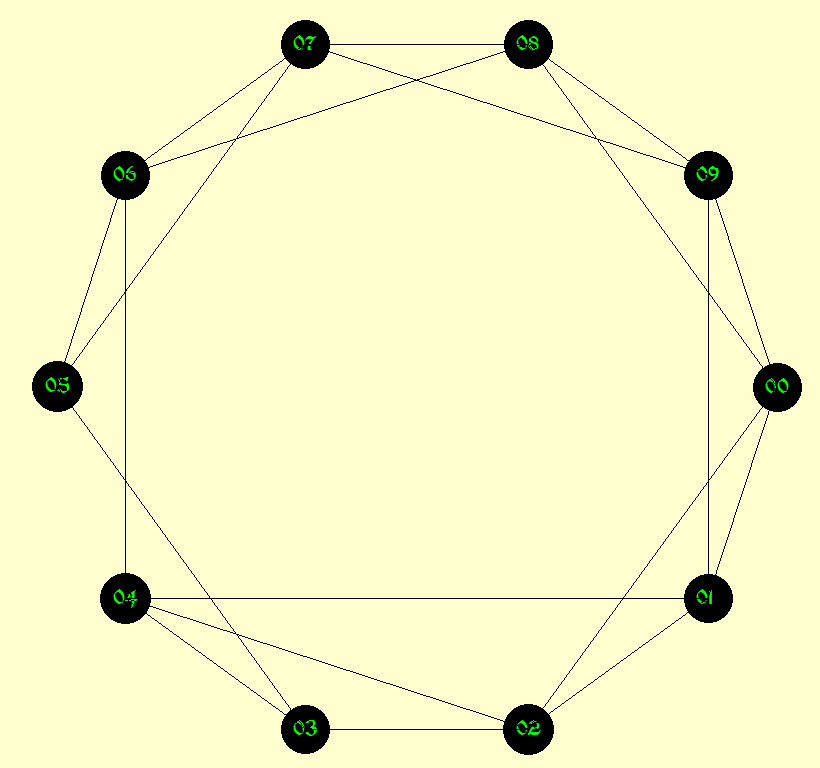
\includegraphics[width= .55\paperwidth]{WSpic.jpg}
\end{figure}
\end{frame}


\section{RandomGraph application}
\begin{frame}{RandomGraph application}{About the application}
"RandomGraph" is an application that allow for visualization of random graphs generated by the three models discussed herein. \\ 
\begin{itemize}
\item Coded in $C^{++}$ using Qt (https://www.qt.io/), used version 5.1.1
\item Consists of 27 files, 14 classes and \textasciitilde4500 SLOC
\item Code compiles with Visual Studio 2010, Service Pack 1.
\item Code compiles with gcc, version 4.8.4 on Ubuntu 14.04 LTS.
\end{itemize}
\end{frame}

\begin{frame}{RandomGraph application}{About the application}

External Dependencies (both are included in the source tree:
\begin{enumerate}
\item {\em pugixml} Used for reading XML files (http://pugixml.org/), used version 1.7.
\item {\em QCustomPlot} Used for generation of histograms (http://qcustomplot.com/), used version 1.3.2.
\end{enumerate}

\end{frame}

\begin{frame}{Where the code lives}
\begin{itemize}
\item Code will be uploaded to a git-hub repository by weeks end.
\item Source for the slides will be included as well (used \LaTeX, with the {\em beamer} package to produce slides.)
\item I will send out mail with the URL
\end{itemize}
\end{frame}

\section{Summary}

\begin{frame}{Summary}

  \begin{itemize}
  \item I introduced the concept of random graphs.
  \item I discussed three models of random graphs, and their potential uses.
  \item I demonstrated the application created to visualize and explore random graphs.
  \end{itemize}

\end{frame}

\begin{frame}{References}
\begin{itemize}   
  \item Erd\"os, P; R\'enyi,A. "On Random Graphs 1". {\em Publicationes mathematicae} \textbf{6}: 290-297 (1959)
  \item Gilbert, E.N. "Random Graphs". {\em Annals of mathematics Statistics"} \textbf{30}(4):1141-1144 (1959)
  \item Watts, Duncan J.; Strogatz,S.H. "Collective dynamics of 'small-world networks' {\em Nature} \textbf{393}(6684): 440-442
  \item Barab\'asi, Albert-L\`aszl\`o. Network Science. Cambridge University Press:Cambridge. 2016 (Chapter 5 available online at http://barabasi.com/f/622.pdf, last acessed 17Jul2016) 
  \item Chung, Fen. "A whirlwind tour of random graphs" (available at: http://www.math.ucsd.edu/~fan/wp/randomg.pdf, last accessed 17Jul2016)

  \end{itemize}
\end{frame}

\begin{frame}{References}
\begin{itemize}
  \item [W2016a]https://en.wikipedia.org/siki/Erd\"os-R\'enyi\_model (last accessed 17Jul2016)
  \item [W2016b]https://en.wikipedia.org/wiki/Watts\_and\_Strogatz\_model (last accessed 17Jul2016)
  \item [W2016c]https://en.wikipedia.org/wik/Barab\'asi-Albert\_model (last accessed 17Jul2016)
  \item [W2015]https://compuzzle.wordpress.com/2015/02/03/generating-barabasi-albert-model-graphs-in-clojure/  
  \end{itemize}
\end{frame}
\end{document}


